\documentclass{article}
\usepackage{amsmath} % need to be on top for eps files
\usepackage{caption}
\usepackage{subcaption}
\usepackage{graphicx}
\graphicspath{ {latex/Images/} }
\usepackage{epstopdf} 


%% sidebyside images


%%%%%%%%%%%%%%%%%%%%%%%%%%%%%%%%%%%%%%%% Create listings (Matlab)
% % Create a matlab listing
\usepackage{listings}
\usepackage{color} %red, green, blue, yellow, cyan, magenta, black, white
\definecolor{mygreen}{RGB}{28,172,0} % color values Red, Green, Blue
\definecolor{mylilas}{RGB}{170,55,241}

\usepackage[utf8]{inputenc}
\usepackage{geometry}
 \geometry{
 a4paper,
 total={175mm,265mm},
 left=15mm,
 top=15mm,
 }
\usepackage{amsmath}%To be able to use split in equation


%%%% Include eps files:
\usepackage{amsmath} % need to be on top for eps files
\usepackage{graphicx}
%set the relative location for eps files
\graphicspath{ {/images/} }
\usepackage{listings}
\usepackage{cleveref} %cleverref needs to stand below amsmath package.
\usepackage{graphicx}
\usepackage{float}
%\usepackage{hyperref}
\usepackage{url} %To be able to use url in references
\usepackage{graphicx}
\usepackage{tabularx} % in the preamble
\usepackage{wrapfig}

\usepackage{algorithm}
\usepackage{algorithmic}


% To get side by side pictures:{
\usepackage{caption}
\usepackage{subcaption}
\usepackage{graphicx}


\usepackage{cleveref} %cleverref needs to stand below amsmath package.
\usepackage{appendix}
\crefname{appsec}{Appendix}{Appendices} % refer to appendix as appendix iso as section (use with text in
\title{Example to plot directly into latex}
%\author{Authors:\\a-t-0}


\date{19-10-2019}
\begin{document}
\crefname{lstlisting}{listing}{listings}
\Crefname{lstlisting}{Listing}{Listings}
%%%%%%%%%%Configure matlab listing%%%%%%%%%%%%%%%%%%
% Specify matlab listing style
\lstset{language=Matlab,%
    %basicstyle=\color{red},
    breaklines=true,%
    morekeywords={matlab2tikz},
    keywordstyle=\color{blue},%
    morekeywords=[2]{1}, keywordstyle=[2]{\color{black}},
    identifierstyle=\color{black},%
    stringstyle=\color{mylilas},
    commentstyle=\color{mygreen},%
    showstringspaces=false,%without this there will be a symbol in the places where there is a space
    numbers=left,%
    numberstyle={\tiny \color{black}},% size of the numbers
    numbersep=9pt, % this defines how far the numbers are from the text
    emph=[1]{for,end,break},emphstyle=[1]\color{red}, %some words to emphasise
    %emph=[2]{word1,word2}, emphstyle=[2]{style},    
}


\maketitle
%\setcounter{chapter}{-1}
\section{Introduction}\label{sec:intro}
% 3 lines max?:) %\newpage
\section{Automated Matlab table}\label{sec:1d}
\begin{table}[H]
\caption{Some table automatically exported from Matlab.}\label{tab:matlab_table}
\centering
\begin{tabular}{|l|l|l|l|l|}
\hline
\input{Tables/table_1.csv}
\end{tabular}
\end{table} %\newpage
\section{Horshoe Orbit}\label{sec:1d}
To find the initial conditions for the asteroid in a horseshoe orbit, one can initialise the orbit without a velocity, in the vicinity of L3. The coordinates of L3 for the given configuration, are: $[-1,000, 0]$\cite{lecture_notes}.
A time-span of 500000 iterations was used. This results in the following horseshoe orbit:
\begin{figure}[H]
    \centering
    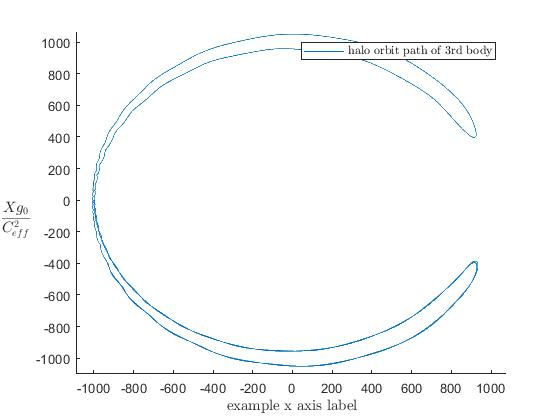
\includegraphics[width=1\textwidth]{Images/plot_1d.jpg}
    \caption{Horseshoe orbit starting near L3}
\end{figure}

\begin{figure}[H]
    \centering
    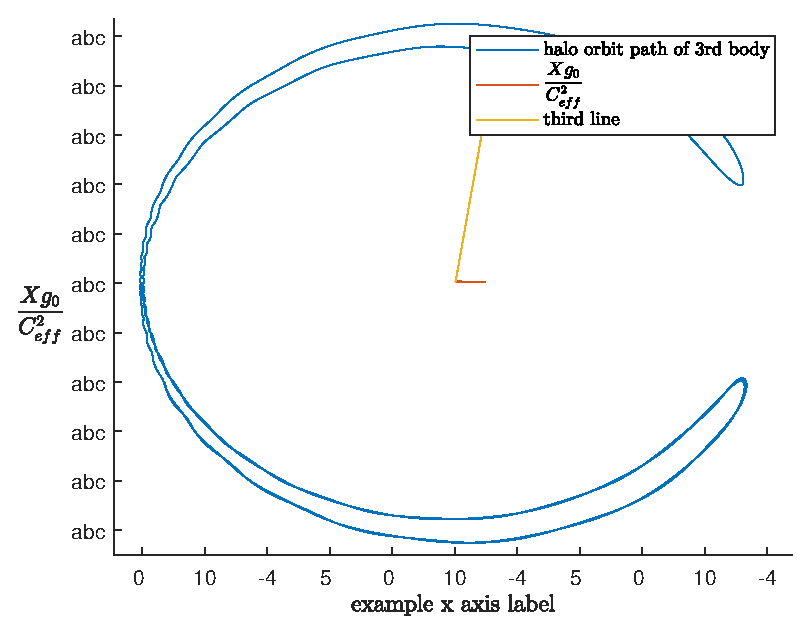
\includegraphics[width=1\textwidth]{Images/plot_1d.eps}
    \caption{Figure consisting of multiple dataseries.}
\end{figure} %\newpage
%\input{Chapters/1h.tex} %\newpage
%\input{Chapters/1i.tex} %\newpage
%\input{Chapters/1j.tex} %\newpage
%\input{Chapters/Conclusion.tex} %\newpage














\bibliographystyle{plain} %plain style
\bibliography{references}
\addcontentsline{toc}{chapter}{Bibliography}


% %\crefname{appsec}{Appendix}{Appendices} % refer to appendix as appendix iso as section
% \crefalias{section}{appsec}
% \begin{appendices}
% \newpage
% \section{Appendix \_\_main\_\_.py}\label{app:1}
\pythonexternal{latex/project3/../../code/project3/src/__main__.py}
% \newpage
% \section{Appendix Main.py}\label{app:2}
\pythonexternal{latex/project3/../../code/project3/src/Main.py}
% \newpage
% \section*{Appendix python code that exports figures to latex}\label{app:3}
\pythonexternal{latex/project3/../../code/project3/src/Plot_to_tex.py}
 \newpage
 \section*{Appendix python code that compiles the latex report to pdf}\label{app:4}
\pythonexternal{latex/project2/../../code/project2/src/Compile_latex.py}
% \newpage
% \section*{Appendix Example Jupyter Notebook}\label{app:6}
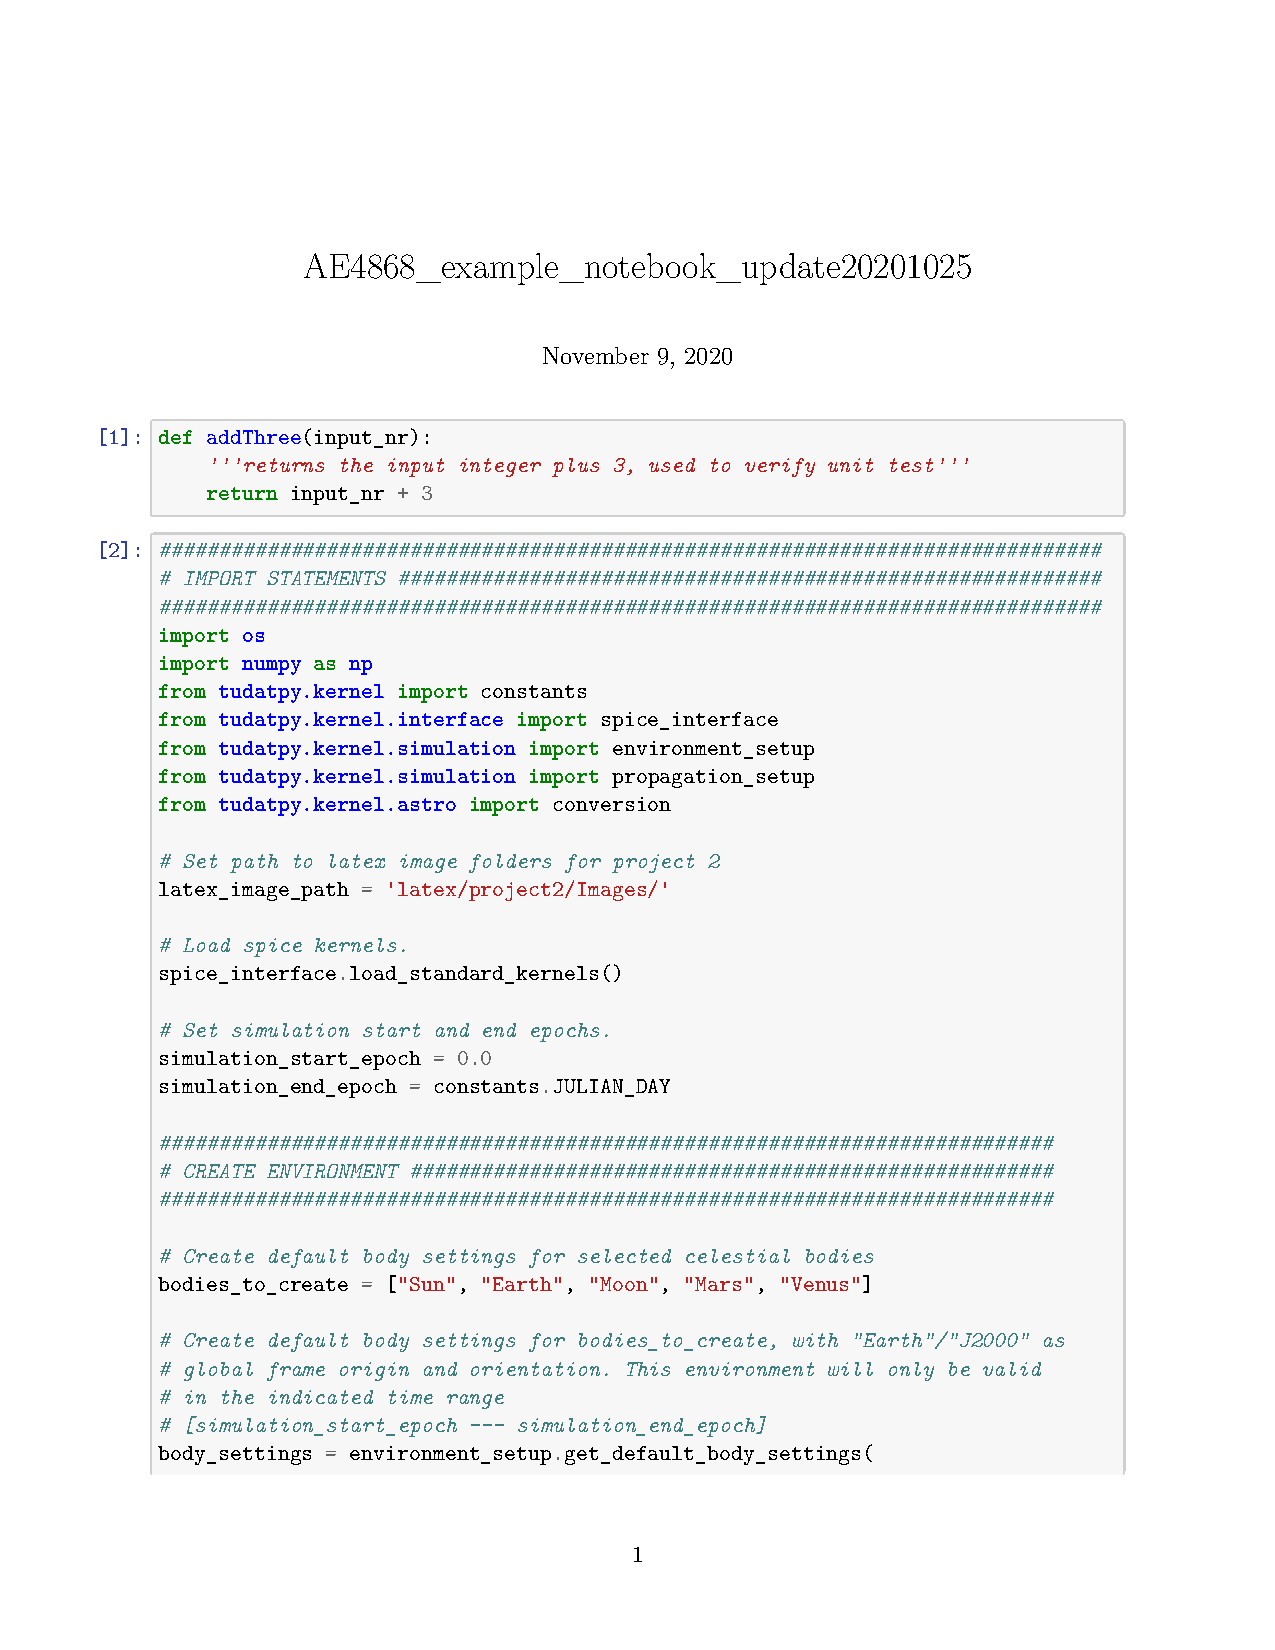
\includepdf[pages=-]{latex/project2/../../code/project2/src/AE4868_example_notebook_update20201025.pdf}
% \end{appendices}

\begin{appendices}
\crefalias{section}{appsec}
\newpage
%\section{Appendix \_\_main\_\_.py}\label{app:1}
\pythonexternal{latex/project3/../../code/project3/src/__main__.py} 
% \newpage
% \section{Appendix Main.py}\label{app:2}
\pythonexternal{latex/project3/../../code/project3/src/Main.py}
% \newpage
% \section*{Appendix python code that exports figures to latex}\label{app:3}
\pythonexternal{latex/project3/../../code/project3/src/Plot_to_tex.py}
% \newpage
% \section*{Appendix python code that compiles the latex report to pdf}\label{app:4}
\pythonexternal{latex/project2/../../code/project2/src/Compile_latex.py}
%\newpage
%\section*{Appendix python code that runs the jupyter notebook(s)}\label{app:5}
\pythonexternal{latex/project3/../../code/project3/src/Run_jupyter_notebooks.py}
\newpage
%\section*{Appendix Example Jupyter Notebook}\label{app:6}
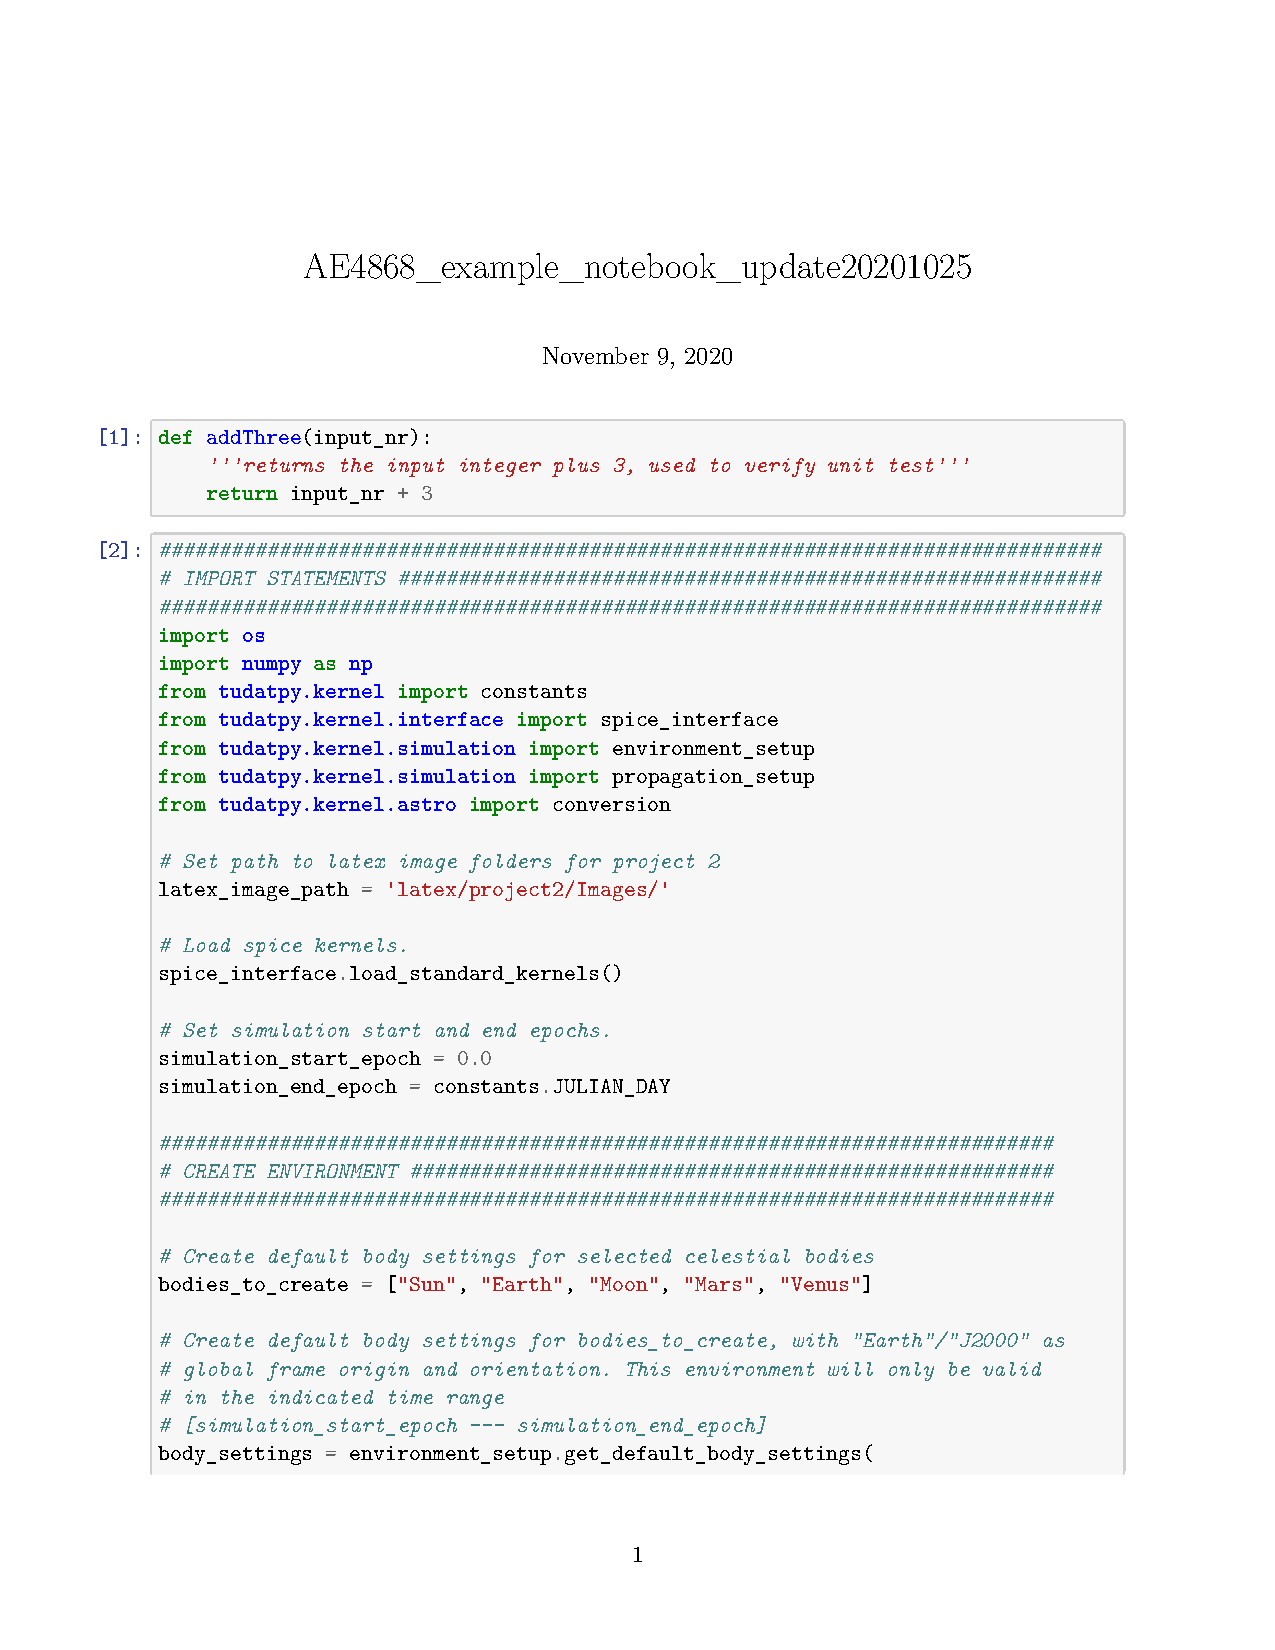
\includepdf[pages=-]{latex/project2/../../code/project2/src/AE4868_example_notebook_update20201025.pdf}
% \input{Appendices/Vuab_art.tex}

\end{appendices}

\end{document}
